\section{Biologische Grundlagen}
In biologischen Systemen bestehen neuronale Netze aus sehr vielen Neuronen und 
Gliazellen. Die Gliazellen dienen der Versorgung, während die Neuronen zur
Übermittlung der Nervenimpulse dienen. Tiere und Menschen besitzen solche Anhäufungen von 
Neuronen, welche über Synapsen miteinander verbunden sind. Ein menschliches 
Gehirn enthält beispielsweise zwischen 30 und 100 Milliarden Neuronen. Neuronen 
können Nervenimpulse selektiv weiterleiten. Durch große Anhäufung und 
Vernetzung mit Nachbarneuronen können so Informationen verarbeitet werden.

\section{Künstliche neuronale Netze}
Künstliche neuronale Netze bestehen aus vielen einzelnen künstlichen Neuronen, 
die - je nach gewählter Strukur - beispielsweise in verschiedenen Schichten
zusammengeschaltet sind. Es gibt die Eingangsschicht, verdeckte Schichten in
der Mitte und die Ausgangsschicht. In der Eingangsschicht sitzen die meisten
Neuronen, die mit allen Eingabeparametern verbunden sind.

Die Neuronen der Eingabeschicht geben ihre Entscheidungen an die verdeckten 
Neuronen weiter und konzentrieren so die Entscheidung. Dann geben sie sie an 
die Neuronen der Ausgabeschicht weiter. Die Neuronen in der Ausgabeschicht 
können nun trainiert werden und geben ihre Schwellwerte dann "`rückwärts"' an 
die vorherigen Neuronen weiter, sogenanntes \textbf{Back-Propagation-Verfahren}. Eine 
künstliche Neuronenzelle "`feuert"' wie eine echte Nervenzelle, wenn die 
Eingabe einen gewissen Schwellwert überschreitet. Jedes Neuron für sich 
genommen ist demnach nicht in der Lage, eine Entscheidung zu fällen - nur in 
der Masse ergibt sich letztlich die richtige Entscheidung. Die folgende 
Abbildung \ref{fig:Neuronales-Netz} zeigt den groben Aufbau eines solchen 
neuronalen Netzes.

\begin{figure}
  \centering
  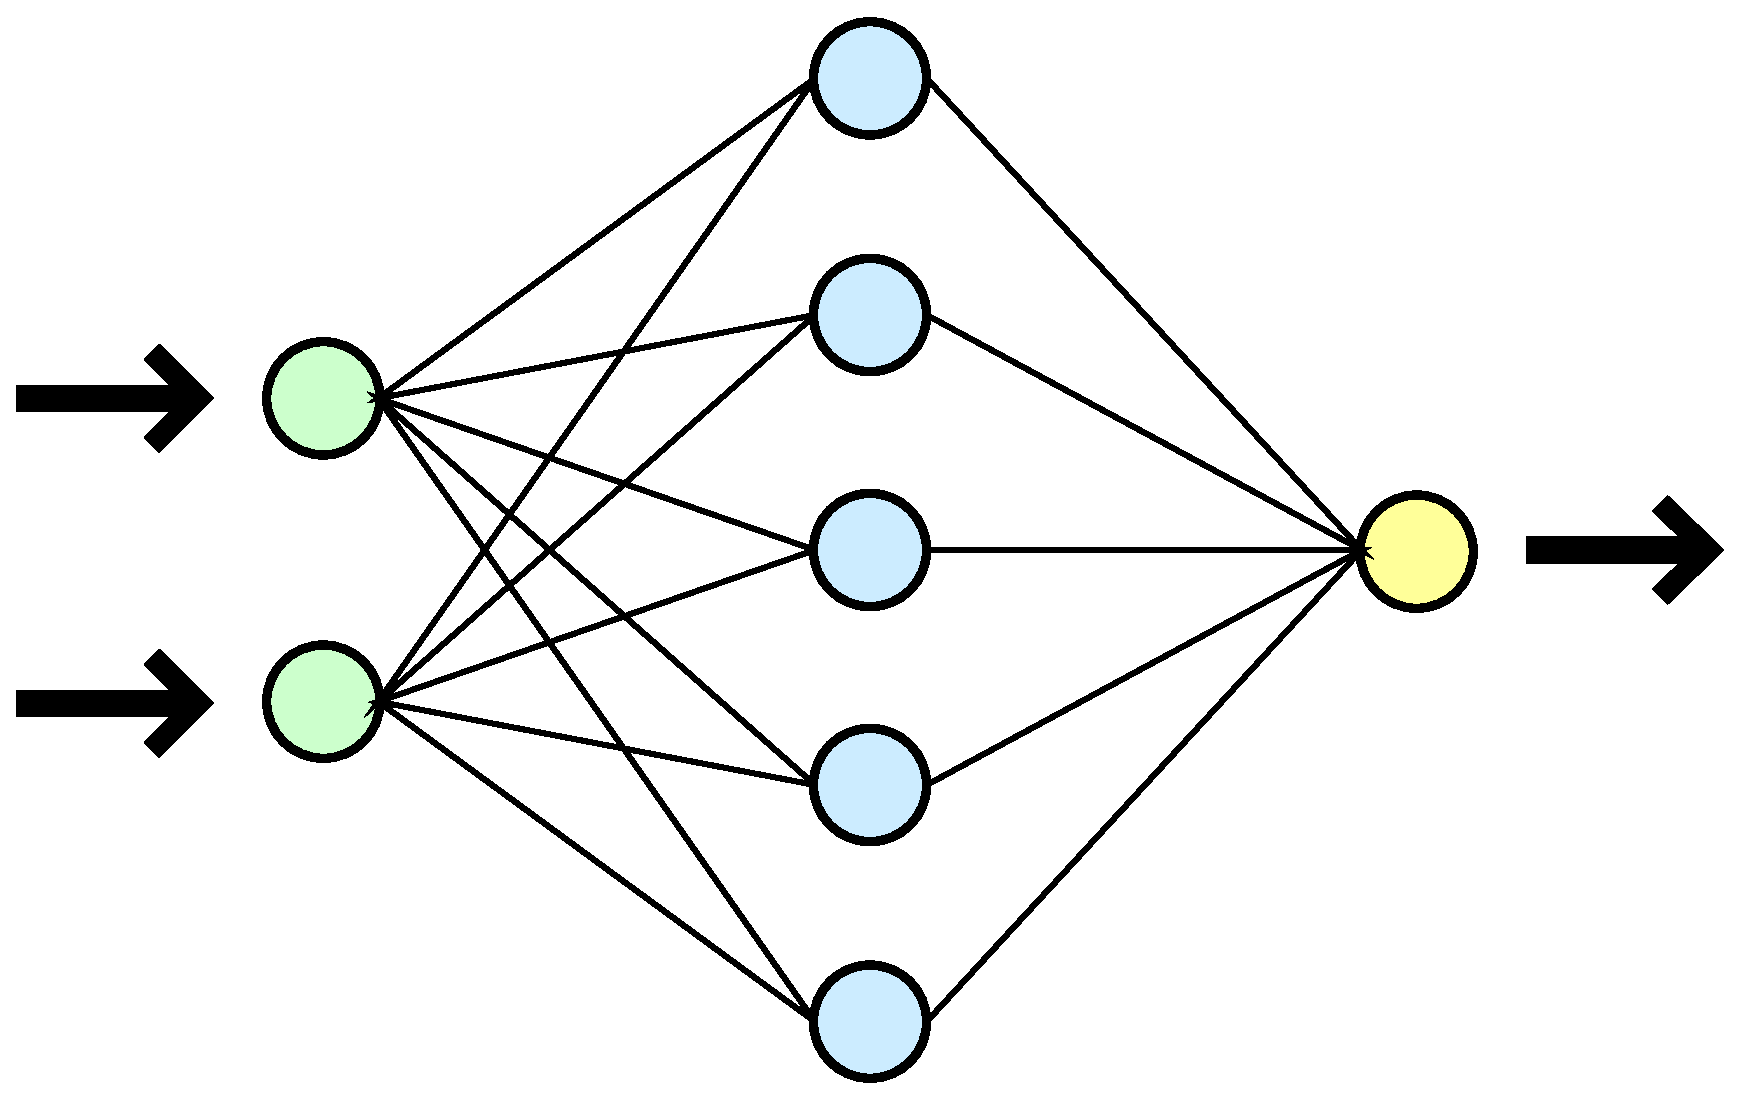
\includegraphics[width=0.8\textwidth]{../images/neuralnetwork.eps}
  \caption{Vereinfachte Darstellung eines künstlichen neuronalen Netzes. 
  Quelle: \cite{wikipedia}}
  \label{fig:Neuronales-Netz}
\end{figure}

Für die Betrachtungen in dieser Arbeit nehmen wir ein künstliches neuronales
Netz vereinfacht als eine Art Blackbox an, welche Eingabedaten $x_i$
entgegennimmt und Ausgabewerte $y_i$ zurückgibt.